\section{Data collection web app}
\label{sec:Data collection web app}
This section introduces several key user logics and algorithms in the data collection web application.
From the user's perspective, the data collection system mainly provides three user processes: new participant registration, participant login and the core function of participant recording and uploading, which are illustrated in Figure \ref{fig:4-webapp-user-register}, \ref{fig:4-webapp-user-login} and \ref{fig:4-webapp-user-record} respectively.

\begin{figure}[!ht]
    \centering
    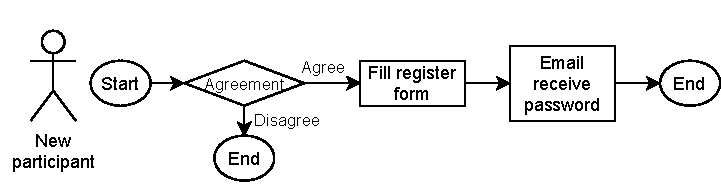
\includegraphics[width=\textwidth]{implementation/imgs/4-webapp-user-register.pdf}
    \caption{New participant registration}
    \label{fig:4-webapp-user-register}
\end{figure}

Figure \ref{fig:4-webapp-user-register} shows the registration process for new participants.
According to the research ethics, each participant needs to clearly understand the research content and provide consent before registering an account.
Another worth mentioning is that the system will generate a random password in the registration process and send it to the email provided by the registrant.
This registration process can prevent the system from collecting users' private passwords.

\begin{figure}[!ht]
    \centering
    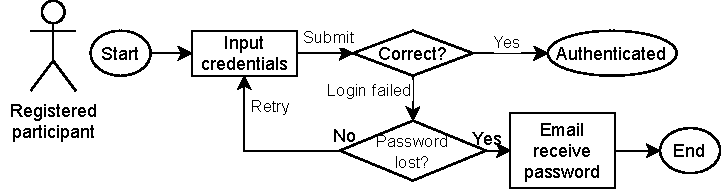
\includegraphics[width=\textwidth]{implementation/imgs/4-webapp-user-login.pdf}
    \caption{Registered participant login}
    \label{fig:4-webapp-user-login}
\end{figure}

After the registration process, Figure \ref{fig:4-webapp-user-login} depicts the authentication process for registered participant.
The participant will input the email address and the random password received during the registration process.
If a participant forgot or lost the random password, he or she can request a new random password and restart the login process.

\begin{figure}[!ht]
    \centering
    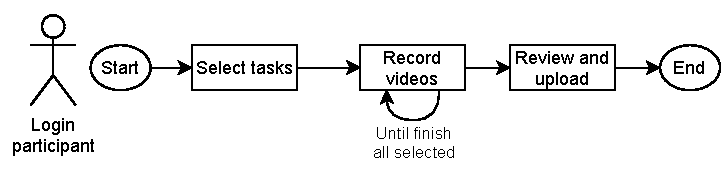
\includegraphics[width=\textwidth]{implementation/imgs/4-webapp-user-record.pdf}
    \caption{Participant recording and uploading}
    \label{fig:4-webapp-user-record}
\end{figure}

Figure \ref{fig:4-webapp-user-record} shows the main workflow of the data collection app after the participant logs in.
In the task selection stage, the web front-end first queries the currently available tasks from the back-end and display them in a list that participant can select.
Each task has detailed text and picture descriptions, which is easy for participants to understand.

After the participant selects desired tasks, the next step is video recording.
The system uses the web real-time communication (WebRTC\footnote{Real-time communication for the web: \url{https://webrtc.org/}}) API provided in most modern browsers to record videos for the participant.
Finally, in the upload step, participants can review each recorded videos and decide whether to upload or try rerecording.

The user registration and login process in the web app adopts a common secure authentication paradigm for online applications.
Algorithm \ref{algo:User authentication} displays the process of user authentication, where the password is double hashed and salted in back-end database storage.
In addition, the system uses short-term-valid JSON Web Tokens (JWT) as the access credentials for RPC calls, also incorporating the mechanism of a periodic token refresh, which further enhances system security and protects users' privacy.

\begin{minipage}{.5\textwidth}
\begin{algorithm}[H]
\caption{User authentication}
\label{algo:User authentication}
\KwData{Email $e$, Password $p$}
\KwResult{Auth $T_a$, Refresh $T_r$}
Web browser front-end:
$EP \gets concat(e, p)$
$h \gets sha256(EP)$
$send(e, h)$\;
\BlankLine
\BlankLine
\BlankLine
\BlankLine
Back-end:
$receive(e, h)$\;
\If{user $e$ does not exist}{
    return error\;
}
\If{bcrypt hash compare $h$ failed}{
    return error\;
}
\tcp{Authenticated}
$T_a \gets JWT(\{userDetail, authUUID\})$\;
$T_r \gets JWT(refreshUUID)$\;
return $T_a, T_r$\;
\end{algorithm}
\end{minipage}
\vline
\begin{minipage}{.5\textwidth}
\begin{algorithm}[H]
\caption{Video uploading}
\label{algo:Video uploading}
\KwData{Blob video data $v$}
\KwResult{Data in chunks $c[x]$}
$s \gets 3 \times 10^{4}$ \tcp*{gRPC 32768 bytes read limit}
\For{$i \gets 0$ \KwTo $\ceil*{\frac{sizeof(v)}{s}}$}{
    $b_{left} \gets i \times s$\;
    $b_{right} \gets \max ((i+1) \times s, sizeof(v))$\;
    $c[i] \gets v[b_{left}:b_{right}]$\;
    $send(i, c[i])$\;
    $progress \gets receive()$\;
    \If{receive progress failed}{
        return error\;
    }
    $updateUI(progress)$\;
    $i \gets i+1$\;
}
\end{algorithm}
\end{minipage}

Algorithm \ref{algo:Video uploading} shows the process for segmenting large video data before uploading it to the backend server.
This segmentation algorithm runs on the browser front end, using \textit{slice} in binary large object (Blob) API for slicing the video.
The communication between the front-end and back-end uses the gRPC bidirectional streaming.
When the front-end uploads data, it also receive acknowledgement and receiving progress from the server.
